\documentclass[10pt,a4paper]{article}
\usepackage[latin1]{inputenc}
\usepackage{amsmath}
\usepackage{amsfonts}
\usepackage{amssymb}
\usepackage{makeidx}
\usepackage{graphicx}
\usepackage{url}
 
\usepackage{geometry}
\geometry{
	a4paper,
	total={170mm,257mm},
	left=20mm,
	top=20mm,
}

\twocolumn

%opening
\title{\textbf{\Huge MimicVR \\
	\Large  Development of Human-Robot Interaction in Virtual Reality Space}}
\author{Santipab Tipparach, Keonwoo Kim, Daniel Ogburn\\
	\textbf{North Dakota State University}\\\textbf{Department of Computer Science}}

\begin{document}
\maketitle


\begin{abstract}

	The main goal of this project is to augment robot movement and decision making using the HTC Vive and a streamlined user interface. This paper will outline the history of virtual reality, why the Vive is the best choice, how robots sensory systems can be drastically improved using the lighthouse tracking system, and how robots and humans can better communicate by transmitting gestures and movement instructions through a virtual reality interface.

\end{abstract}

	\section{Introduction}
	Virtual reality is a powerful tool in the worlds of data analysis and immersive simulations. The HTC Vive introduces a method of entering virtual reality and capturing a user's precise movements. This is all possible using the HTC Vive's light house technology, which provides sub-millimeter positional accuracy. There has been some work already done introducing robots to the virtual world, however this project takes some of the projects found online and takes it a step further. On the website Hackaday.com, many projects are outlined \cite{hack1}. This includes a project that was very like our initial setup, however the project on the website was a very small scope and was surpassed by this project on the first weekend. Another project demonstrated the power of augmentation by tracking a drone in a virtual space and using this technology to swap batteries quickly on a base and fly for another fifteen minutes. This project will utilize the Vive tool, the Elegoo robot kit, and a central CPU/GPU to render, simulate, and send instructions via Bluetooth from a virtual environment to the physical robot.

	\section{Background}
	In the past, robots used various techniques for tracking and motion sensors such as line tracking, IMU(Inertia Measurement Unity), ultra sonic, and various methods for sampling points with depth. One of the biggest challenges of positional tracking is that the positional coordinates of each tracked object is best used in relation to another object, it becomes difficult for the tracked object to work on it's own by only sensing the environment.
	\\
	In GPS technology, an array of satellites orbit the earth to help triangulate a position in a 3D spatial coordinate system using the time differences each satellite is from the center point \cite{gizmodo1}. For a very long time, the few feet of inaccuracy was tolerated for large scale navigation (moving over vast distances of miles). However, when it comes to tracking at the finer scale, the human scale, we cannot use GPS for close range, high precision tracking.
	\\
	The HTC Vive, released in April 2016 \cite{techradar1}, provides room scale tracking with high accuracy. Mainly used for Virtual Reality, this project will utilize this advantage to harness that accuracy into encoding instructions and providing robots with human like tasks. Upon solving the issues of precision, simulations can be designed and algorithms can be tested all using the virtual space.
	\\
	In addition to high accuracy tracking, VR also allows for a safe and cost effective space for testing out various situations for robotic behaviors. An example of this maybe in a hazardous environment\cite{Bugalia} with lethal radiation or a potential bomb threat\cite{Codd-Downey}. This main reason alone, combined with certain time critical tasks can utilize the power of VR not only to simulate, but allow operators to interface with the robot in realtime in a safe environment. Long past are the days of joystick controls for operating analog robots. With the advent of VR controls, robots not only mimic human behavior but can actually learn to do better than their human counter parts and in turn, humans can learn from those robots as well.
	
	\section{Description}
	TODO: move some of the methodoloy up here.
	\section{System Description}
	TODO: Describe system architecture and how the networking system is setup
	\section{Experimentation}
	This study examines the use of VR as an interface tool for robotics. The main question here is, how can Virtual Reality technology be used to augment the simulation and command of physical robots? The environment will be set up in Unity with the SteamVR software installed. It is also using the VR toolkit from the Unity asset store which is free.
	\\
	To simulate robotic systems, a Unity rigid body object is assigned to a simulated version. 		\begin{figure}[h]
		\centering
		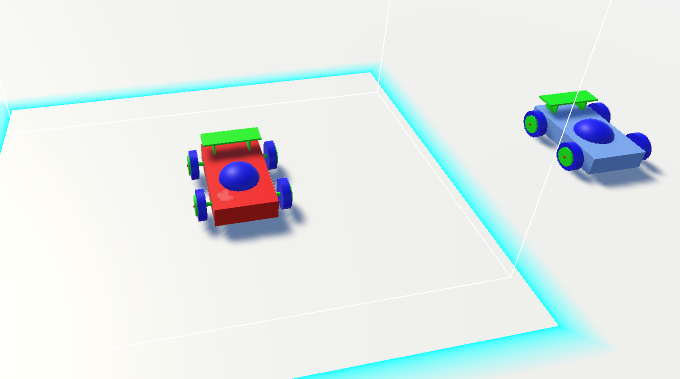
\includegraphics[width=.4\textwidth]{robot-rivalry.png}
		\caption{Two robots competing to execute behavioral algorithms, the physical (left) and the virtual (right).}
		\label{fig:robot-rivalry}
	\end{figure}
	The main implementation feature of the project will be the simulation code. With the infrastructure to relay data from the positional tracker from the robot to the desktop, and the desktop runs a simulation that will send back data, a script can be quickly written to provide different behavior systems to run using a secondary tracker.
	\\
	Basic instructions can be encoded such as moving in a circular motion once, and then will be translated to both robot models, the physical and virtual simultaneously. This allows for data collection and analysis of the difference in the algorithm used for the physical and virtual counterparts. In addition data can be collected in terms of delta-rotational and delta-velocities to determine correct orientation and speed using timed outputs of movement commands.
	\\
	This feedback loop is ideal for a PID(Partial Integral Derivative) controller that can be used to drive both models simultaneously. Certain factors such as friction have to be accounted for in order to have these two models operate in a relatively similar fashion. The PID controller will allow the robots to gain full control of speed and directional heading to a close approximation to the desired rotation and velocity. This will allow the robots to hit targeted way points without any external guidance.
	\\
	Experiments will be designed to test out various user-to-robot interfaces such as commanding the robot to follow a designated way point. Sets of different waypoints will be used to test the PID system and its parameters. Some adaptive learning techniques maybe applied so that the robot can calibrate itself on various terrains.
	\\
	The first stage of experiments will be to test out the capability of following multiple way points in 2 dimensional space. These will include, single way point navigation, multiple way point navigation, and simulated collision avoidance.
	\\
	The second stage of experiments will be designed to test out 3 dimensional movements. While this will still be used on a wheeled robot, the robots will still have portions in the simulation that can move in the Y-Axis (Unity uses the left hand coordinate system with Y as up/down). This should allow a robot to follow the movements of the secondary tracked object with high precision using the PID system and the high accuracy tracking system of the Vive.
	
	
	
	\section*{REFERENCES}
	\begin{thebibliography}{99}
		
		\bibitem{hack1}{Cameron Coward, ''HTC Vive Gives Autonomous Robots Direction'',\url{http://hackaday.com/2016/08/23/htc-vive-gives-autonomous-robots-direction/},2016.}
		
			
		\bibitem{gizmodo1}{Sean Buckley, ''This Is How Valve?s Amazing Lighthouse Tracking Technology Works'',\url{http://gizmodo.com/this-is-how-valve-s-amazing-lighthouse-tracking-technol-1705356768},2016.}
		
	
		\bibitem{techradar1}{Jon Porter, ''This Is How Valve?s Amazing Lighthouse Tracking Technology Works'',\url{http://www.techradar.com/news/htc-vive-2-release-date-news-and-rumors}, 2017.}
		
		\bibitem{Bugalia}{Nishant Bugalia et. al., ''Immersive environment for robotic tele-operations'', 2015.}
		
		
		\bibitem{Codd-Downey}{Robert Codd-Downey and Michael Jenkin, ''Crime Scene Robot and Sensor Simulation'', 2009.}
		
		
	\end{thebibliography}
\end{document}
